
%% sasmoota2017.tex
%% V0.1
%% 26.01.2017
%% by Eveliina Pakarinen
%%
%% This is a skeleton file demonstrating the use of IEEEtran.cls
%% (requires IEEEtran.cls version 1.8b or later) with an IEEE
%% conference paper.


%%*************************************************************************
%% Legal Notice:
%% This code is offered as-is without any warranty either expressed or
%% implied; without even the implied warranty of MERCHANTABILITY or
%% FITNESS FOR A PARTICULAR PURPOSE! 
%% User assumes all risk.
%% In no event shall the IEEE or any contributor to this code be liable for
%% any damages or losses, including, but not limited to, incidental,
%% consequential, or any other damages, resulting from the use or misuse
%% of any information contained here.
%%
%% All comments are the opinions of their respective authors and are not
%% necessarily endorsed by the IEEE.
%%
%% This work is distributed under the LaTeX Project Public License (LPPL)
%% ( http://www.latex-project.org/ ) version 1.3, and may be freely used,
%% distributed and modified. A copy of the LPPL, version 1.3, is included
%% in the base LaTeX documentation of all distributions of LaTeX released
%% 2003/12/01 or later.
%% Retain all contribution notices and credits.
%% ** Modified files should be clearly indicated as such, including  **
%% ** renaming them and changing author support contact information. **
%%*************************************************************************


% *** Authors should verify (and, if needed, correct) their LaTeX system  ***
% *** with the testflow diagnostic prior to trusting their LaTeX platform ***
% *** with production work. The IEEE's font choices and paper sizes can   ***
% *** trigger bugs that do not appear when using other class files.       ***                          ***
% The testflow support page is at:
% http://www.michaelshell.org/tex/testflow/



\documentclass[conference]{sasmoota2017}
% Some Computer Society conferences also require the compsoc mode option,
% but others use the standard conference format.


% Some very useful LaTeX packages include:
% (uncomment the ones you want to load)


% *** MISC UTILITY PACKAGES ***
%
%\usepackage{ifpdf}
% Heiko Oberdiek's ifpdf.sty is very useful if you need conditional
% compilation based on whether the output is pdf or dvi.
% usage:
% \ifpdf
%   % pdf code
% \else
%   % dvi code
% \fi
% The latest version of ifpdf.sty can be obtained from:
% http://www.ctan.org/pkg/ifpdf
% Also, note that IEEEtran.cls V1.7 and later provides a builtin
% \ifCLASSINFOpdf conditional that works the same way.
% When switching from latex to pdflatex and vice-versa, the compiler may
% have to be run twice to clear warning/error messages.






% *** CITATION PACKAGES ***
%
%\usepackage{cite}
% cite.sty was written by Donald Arseneau
% V1.6 and later of IEEEtran pre-defines the format of the cite.sty package
% \cite{} output to follow that of the IEEE. Loading the cite package will
% result in citation numbers being automatically sorted and properly
% "compressed/ranged". e.g., [1], [9], [2], [7], [5], [6] without using
% cite.sty will become [1], [2], [5]--[7], [9] using cite.sty. cite.sty's
% \cite will automatically add leading space, if needed. Use cite.sty's
% noadjust option (cite.sty V3.8 and later) if you want to turn this off
% such as if a citation ever needs to be enclosed in parenthesis.
% cite.sty is already installed on most LaTeX systems. Be sure and use
% version 5.0 (2009-03-20) and later if using hyperref.sty.
% The latest version can be obtained at:
% http://www.ctan.org/pkg/cite
% The documentation is contained in the cite.sty file itself.






% *** GRAPHICS RELATED PACKAGES ***
%
\ifCLASSINFOpdf
  % \usepackage[pdftex]{graphicx}
  % declare the path(s) where your graphic files are
  % \graphicspath{{../pdf/}{../jpeg/}}
  % and their extensions so you won't have to specify these with
  % every instance of \includegraphics
  % \DeclareGraphicsExtensions{.pdf,.jpeg,.png}
\else
  % or other class option (dvipsone, dvipdf, if not using dvips). graphicx
  % will default to the driver specified in the system graphics.cfg if no
  % driver is specified.
  % \usepackage[dvips]{graphicx}
  % declare the path(s) where your graphic files are
  % \graphicspath{{../eps/}}
  % and their extensions so you won't have to specify these with
  % every instance of \includegraphics
  % \DeclareGraphicsExtensions{.eps}
\fi
% graphicx was written by David Carlisle and Sebastian Rahtz. It is
% required if you want graphics, photos, etc. graphicx.sty is already
% installed on most LaTeX systems. The latest version and documentation
% can be obtained at: 
% http://www.ctan.org/pkg/graphicx
% Another good source of documentation is "Using Imported Graphics in
% LaTeX2e" by Keith Reckdahl which can be found at:
% http://www.ctan.org/pkg/epslatex
%
% latex, and pdflatex in dvi mode, support graphics in encapsulated
% postscript (.eps) format. pdflatex in pdf mode supports graphics
% in .pdf, .jpeg, .png and .mps (metapost) formats. Users should ensure
% that all non-photo figures use a vector format (.eps, .pdf, .mps) and
% not a bitmapped formats (.jpeg, .png). The IEEE frowns on bitmapped formats
% which can result in "jaggedy"/blurry rendering of lines and letters as
% well as large increases in file sizes.
%
% You can find documentation about the pdfTeX application at:
% http://www.tug.org/applications/pdftex





% *** MATH PACKAGES ***
%
%\usepackage{amsmath}
% A popular package from the American Mathematical Society that provides
% many useful and powerful commands for dealing with mathematics.
%
% Note that the amsmath package sets \interdisplaylinepenalty to 10000
% thus preventing page breaks from occurring within multiline equations. Use:
%\interdisplaylinepenalty=2500
% after loading amsmath to restore such page breaks as IEEEtran.cls normally
% does. amsmath.sty is already installed on most LaTeX systems. The latest
% version and documentation can be obtained at:
% http://www.ctan.org/pkg/amsmath





% *** SPECIALIZED LIST PACKAGES ***
%
%\usepackage{algorithmic}
% algorithmic.sty was written by Peter Williams and Rogerio Brito.
% This package provides an algorithmic environment fo describing algorithms.
% You can use the algorithmic environment in-text or within a figure
% environment to provide for a floating algorithm. Do NOT use the algorithm
% floating environment provided by algorithm.sty (by the same authors) or
% algorithm2e.sty (by Christophe Fiorio) as the IEEE does not use dedicated
% algorithm float types and packages that provide these will not provide
% correct IEEE style captions. The latest version and documentation of
% algorithmic.sty can be obtained at:
% http://www.ctan.org/pkg/algorithms
% Also of interest may be the (relatively newer and more customizable)
% algorithmicx.sty package by Szasz Janos:
% http://www.ctan.org/pkg/algorithmicx




% *** ALIGNMENT PACKAGES ***
%
%\usepackage{array}
% Frank Mittelbach's and David Carlisle's array.sty patches and improves
% the standard LaTeX2e array and tabular environments to provide better
% appearance and additional user controls. As the default LaTeX2e table
% generation code is lacking to the point of almost being broken with
% respect to the quality of the end results, all users are strongly
% advised to use an enhanced (at the very least that provided by array.sty)
% set of table tools. array.sty is already installed on most systems. The
% latest version and documentation can be obtained at:
% http://www.ctan.org/pkg/array


% IEEEtran contains the IEEEeqnarray family of commands that can be used to
% generate multiline equations as well as matrices, tables, etc., of high
% quality.




% *** SUBFIGURE PACKAGES ***
%\ifCLASSOPTIONcompsoc
%  \usepackage[caption=false,font=normalsize,labelfont=sf,textfont=sf]{subfig}
%\else
%  \usepackage[caption=false,font=footnotesize]{subfig}
%\fi
% subfig.sty, written by Steven Douglas Cochran, is the modern replacement
% for subfigure.sty, the latter of which is no longer maintained and is
% incompatible with some LaTeX packages including fixltx2e. However,
% subfig.sty requires and automatically loads Axel Sommerfeldt's caption.sty
% which will override IEEEtran.cls' handling of captions and this will result
% in non-IEEE style figure/table captions. To prevent this problem, be sure
% and invoke subfig.sty's "caption=false" package option (available since
% subfig.sty version 1.3, 2005/06/28) as this is will preserve IEEEtran.cls
% handling of captions.
% Note that the Computer Society format requires a larger sans serif font
% than the serif footnote size font used in traditional IEEE formatting
% and thus the need to invoke different subfig.sty package options depending
% on whether compsoc mode has been enabled.
%
% The latest version and documentation of subfig.sty can be obtained at:
% http://www.ctan.org/pkg/subfig




% *** FLOAT PACKAGES ***
%
%\usepackage{fixltx2e}
% fixltx2e, the successor to the earlier fix2col.sty, was written by
% Frank Mittelbach and David Carlisle. This package corrects a few problems
% in the LaTeX2e kernel, the most notable of which is that in current
% LaTeX2e releases, the ordering of single and double column floats is not
% guaranteed to be preserved. Thus, an unpatched LaTeX2e can allow a
% single column figure to be placed prior to an earlier double column
% figure.
% Be aware that LaTeX2e kernels dated 2015 and later have fixltx2e.sty's
% corrections already built into the system in which case a warning will
% be issued if an attempt is made to load fixltx2e.sty as it is no longer
% needed.
% The latest version and documentation can be found at:
% http://www.ctan.org/pkg/fixltx2e


%\usepackage{stfloats}
% stfloats.sty was written by Sigitas Tolusis. This package gives LaTeX2e
% the ability to do double column floats at the bottom of the page as well
% as the top. (e.g., "\begin{figure*}[!b]" is not normally possible in
% LaTeX2e). It also provides a command:
%\fnbelowfloat
% to enable the placement of footnotes below bottom floats (the standard
% LaTeX2e kernel puts them above bottom floats). This is an invasive package
% which rewrites many portions of the LaTeX2e float routines. It may not work
% with other packages that modify the LaTeX2e float routines. The latest
% version and documentation can be obtained at:
% http://www.ctan.org/pkg/stfloats
% Do not use the stfloats baselinefloat ability as the IEEE does not allow
% \baselineskip to stretch. Authors submitting work to the IEEE should note
% that the IEEE rarely uses double column equations and that authors should try
% to avoid such use. Do not be tempted to use the cuted.sty or midfloat.sty
% packages (also by Sigitas Tolusis) as the IEEE does not format its papers in
% such ways.
% Do not attempt to use stfloats with fixltx2e as they are incompatible.
% Instead, use Morten Hogholm'a dblfloatfix which combines the features
% of both fixltx2e and stfloats:
%
% \usepackage{dblfloatfix}
% The latest version can be found at:
% http://www.ctan.org/pkg/dblfloatfix




% *** PDF, URL AND HYPERLINK PACKAGES ***
%
%\usepackage{url}
% url.sty was written by Donald Arseneau. It provides better support for
% handling and breaking URLs. url.sty is already installed on most LaTeX
% systems. The latest version and documentation can be obtained at:
% http://www.ctan.org/pkg/url
% Basically, \url{my_url_here}.




% *** Do not adjust lengths that control margins, column widths, etc. ***
% *** Do not use packages that alter fonts (such as pslatex).         ***
% There should be no need to do such things with IEEEtran.cls V1.6 and later.
% (Unless specifically asked to do so by the journal or conference you plan
% to submit to, of course. )

\usepackage{graphicx}
\usepackage[export]{adjustbox}

% correct bad hyphenation here
\hyphenation{op-tical net-works semi-conduc-tor}


\begin{document}
%
% paper title
% Titles are generally capitalized except for words such as a, an, and, as,
% at, but, by, for, in, nor, of, on, or, the, to and up, which are usually
% not capitalized unless they are the first or last word of the title.
% Linebreaks \\ can be used within to get better formatting as desired.
% Do not put math or special symbols in the title.
\title{Multi-tenancy in scientific literature from Software as a Service perspective}


% author names and affiliations
% use a multiple column layout for up to three different
% affiliations
\author{\IEEEauthorblockN{Eveliina Pakarinen}
\IEEEauthorblockA{Department of Computer Science \\
University of Helsinki\\
Email: eveliina.pakarinen@helsinki.fi}}


% make the title area
\maketitle

% As a general rule, do not put math, special symbols or citations
% in the abstract
\begin{abstract}

Multi-tenancy is a high level architectural pattern which can be used in cloud computing environment when offering applications using Software as a Service business model. In multi-tenancy pattern service provider hosts a single instance of an application on his or her infrastructure. This application is accessed by multiple customers, so-called tenants. Tenants share the resources of the infrastructure. Multi-tenancy is still a relatively new topic in scientific literature. The research domain of multi-tenancy is not yet mature which can be seen from the lack of industrial experience reports on multi-tenancy. The use of multi-tenancy pattern brings multiple benefits both to the service provider and to the customers. In addition to the benefits there are also some challenges that affect the use of multi-tenancy. In this paper the different variants of multi-tenancy in scientific literature are investigated from the perspective of Software as a Service business model. The connection between Software as a Service and multi-tenancy is also investigated. Finally some challenges caused by the characteristics of multi-tenancy are presented. 

\end{abstract}

% no keywords

Keywords: multi-tenancy, Software as a Service, definition of multi-tenancy



\IEEEpeerreviewmaketitle



\section{Introduction}

\textit{Software as a Service (SaaS)} is a novel business model where software and the underlying ICT infrastructure are offered as an on-demand service for customers through Internet \cite{Bezemer:2010:MaintenanceDream}. In Software as a Service business model the service provider maintains the application and offers the software as a service to the customers \cite{Bezemer:2010:MaintenanceDream}. By using software offered by a third party service provider companies can use various ICT services without maintaining or purchasing their own ICT infrastructure \cite{Bezemer:2010:MaintenanceDream}. 

\textit{Multi-tenancy} is a high level architectural pattern which can be used when offering applications as Software as a Service in cloud computing environment \cite{Kabbedijk2015:Defining}. In multi-tenancy pattern the service provider hosts a single instance of the software product on his or her infrastructure and multiple customers, so-called tenants, access the same instance of the software \cite{Bezemer:2010:MaintenanceDream}. The definition for a tenant is: \textit{"A tenant is the organizational entity which rents a multi-tenant SaaS solution"} \cite{Bezemer:2010:MaintenanceDream}. A tenant groups typically multiple users of the same organization and these users are the stakeholders in the organization \cite{Bezemer:2010:MaintenanceDream}. 

There are multiple benefits for the service provider when using multi-tenant architecture pattern when implementing Software as a Service applications. The first benefit is that the application deployment becomes easier because only one application instance has to be deployed \cite{Bezemer:2010:MaintenanceDream}. In multi-tenancy multiple customers access the same software instance and they do not need own dedicated instance of the software. This means that the customers share the same hardware resources when using multi-tenant Software as a Service application \cite{Guo:2007:FrameworkForNative}. That increases and improves the utilization rate of the hardware which is the second benefit of the multi-tenancy \cite{Bezemer:2010:MaintenanceDream}. 

These two benefits reduce service provider's overall delivery costs of the application \cite{Bezemer:2010:MaintenanceDream}. The reduced delivery costs of a multi-tenant application can help improve service provider's profit margin \cite{Guo:2007:FrameworkForNative}. The reduced delivery costs make it possible for the service provider to offer the service to the customers at lower service subscription costs \cite{Guo:2007:FrameworkForNative}. The reduced overall costs of a multi-tenant application make multi-tenant applications interesting for customers in the small and medium enterprise (SME) segment of the market \cite{Bezemer:2010:MaintenanceDream}.

When describing multi-tenancy in scientific literature the three often mentioned characteristics are sharing of hardware resources, possibility to configure the shared application instance in runtime and shared application and database instance. Those characteristics are also part of the definition of multi-tenancy which is used in this seminar paper. 

In addition to the benefits of multi-tenancy there are also some challenges that come with the use of multi-tenancy. Challenges can arise in the application development, deployment and management phases \cite{Guo:2007:FrameworkForNative}. The three characteristics of multi-tenancy can cause some of the challenges of multi-tenancy. Areas where challenges can arise are for example in application performance, maintenance and in security \cite{Bezemer:2010:MaintenanceDream}. 

Multi-tenancy is still a relatively new topic in scientific literature in the domain of software and hardware systems \cite{Kabbedijk2015:Defining}. The term \textit{'multi-tenancy'} was explicitly mentioned for the first time in a scientific paper in year 2006 \cite{Kabbedijk2015:Defining, Carraro:2006:ArchitectureLongTail}. Since then many definitions for multi-tenancy have been proposed \cite{Kabbedijk2015:Defining}. Also many solutions related to implementing multi-tenancy have been proposed in the multi-tenancy research over the years but there has been very few industrial reports about experiences on multi-tenancy \cite{Kabbedijk2015:Defining}. 

The low amount of industrial reports on multi-tenancy indicates that the research domain of multi-tenancy is not yet mature and that the proposed solutions have not yet been implemented or evaluated \cite{Kabbedijk2015:Defining}. The high amount of proposals and the low amount of industrial reports can also indicate that there is a lack of cooperation between industry and academia in multi-tenancy research domain \cite{Kabbedijk2015:Defining}.

In this paper the different variants of multi-tenancy in scientific literature are investigated from the perspective of Software as a Service business model. The connection between Software as a Service business model and multi-tenancy is also investigated. Finally some possible challenges caused by the characteristics of multi-tenancy are presented.

This paper is organized as follows. In Section 2 the research questions and the research methods for data collection for this paper are presented. In section 3 the different variants of multi-tenancy are presented from the viewpoint of a Software as a Service business model. In section 4 the characteristics of multi-tenancy and some challenges caused by those characteristics are presented. In section 5 the answers to the research questions are discussed. The paper is concluded section 6. 




%\cite{Kabbedijk2015:Defining}
%\cite{Bezemer:2010:MaintenanceDream}
%\cite{Weissman:2009:Forcecom}
%\cite{Guo:2007:FrameworkForNative}
%\cite{Kang:2011:DesignOfConceptual}
%\cite{Pal:2015:ApplicationMultiTenancy}
%\cite{Schroeter:2012:TowardsModeling}
%\cite{Samrajesh:2016:ScalableComponent}
%\cite{Bien:2015:MultiTenantWebApp}
%\cite{Bezemer:2010:EnablingMultiTenancy}
%\cite{Ru:2014:SoftareEngineering}
%\cite{Vidhyalakshmi:2014:DesignComparison}
%\cite{Mietzner:2009:VariabilityModeling}
%\cite{Carraro:2006:ArchitectureLongTail}
%\cite{Chong:2006:MultiTenantDataArchitecture}




\section{Research questions and methods for data collection}

This seminar paper tries to provide a description of the different variants of multi-tenancy in scientific literature from the perspective of Software as a Service business model. The main research questions for this seminar paper are: 
\begin{enumerate}
\item How multi-tenancy is defined in scientific literature?
\item Is there a connection between multi-tenancy and Software as a Service business model?
\item What challenges the characteristics of multi-tenancy can cause?
\end{enumerate}

The work in this seminar paper is based on academic papers and technical articles. The topic for this seminar paper was found during a search for papers for a different topic. The initial article which inspired the topic of this seminar paper was \textit{"Multi-Tenant Web Application Framework Architecture Pattern"} by Bien and Thu \cite{Bien:2015:MultiTenantWebApp}. After learning about multi-tenancy for the first time from this article the search for papers about multi-tenancy continued in the ACM Digital Library and in the IEEE Xplore Digital Library. 

The search was done with quick search using combinations and different variations of words \textit{'multi-tenancy'} or \textit{'multi-tenant'} with or without '-'-character and \textit{'SaaS'} or \textit{'Software as a Service'} and \textit{'architecture'}. After getting the results from the search the results were refined by setting the range of publication year from 2014 to 2016. After finding a couple of papers that discussed multi-tenancy the references in those papers were used to find more papers related to the topic. Web of Science was also used to find papers that had cited the papers found during the search in digital libraries.

The initial goal for data collection was to find as many papers as possible. After that the first thing to do was to filter out papers that were not suitable as sources for this seminar paper. Characteristics for not suitable papers were for example that the paper was published in a too small conference or in an unknown journal or that it did not discuss multi-tenancy in application level in Software as a Service applications or that multi-tenancy was not discussed from architectural perspective. 

After that the remaining papers were organized to four groups based on the abstract, introduction and conclusion parts of the papers. The groups in which the papers were organized were: 
\begin{enumerate}
\item not so relevant papers for this seminar work
\item probably important papers for this seminar work
\item papers that propose some multi-tenant pattern or architecture
\item supporting papers with relevant background information.
\end{enumerate}
The papers that belonged to group 1 were left out and the papers that belonged to groups 2, 3 and 4 were studied further. The references that are used in this seminar paper are based on the papers that belonged to groups 2, 3 and 4. 


\section{Variants of multi-tenancy in scientific literature}

\subsection{The definition of multi-tenancy}


Multi-tenancy is a high level architectural pattern which can be used to share computing resources when offering software products using Software as a Service business model \cite{Kabbedijk2015:Defining}. In multi-tenancy a single instance of an application is hosted on service provider's infrastructure \cite{Kabbedijk2015:Defining}. This single instance is accessed by multiple tenants and can be customized according to the requirements of different tenants \cite{Kabbedijk2015:Defining}. Multi-tenancy has evolved from previous information technology paradigms like time-sharing, application service provider (ASP) model and multi-user model \cite{Kabbedijk2015:Defining}. Multi-tenancy was explicitly mentioned in scientific literature for the first time in the domain of software and hardware systems in year 2006 \cite{Kabbedijk2015:Defining, Carraro:2006:ArchitectureLongTail}. 

In academic literature the definition of multi-tenancy has been varying and there has been differences in the interpretation of multi-tenancy among academics in academia \cite{Kabbedijk2015:Defining}. In order to chart and bridge the varying definitions of multi-tenancy and to provide an overview of the multi-tenancy domain Kabbedijk et al. \cite{Kabbedijk2015:Defining} performed a structural search in academic literature and in public blog posts. 

As a result of their structural search Kabbedijk et al. proposed a comprehensive definition for multi-tenancy which is based on 43 different definitions of multi-tenancy presented in academic literature \cite{Kabbedijk2015:Defining}. The definition which Kabbedijk et al. proposed for multi-tenancy is: \textit{"Multi-tenancy is a property of a system where multiple customers, so-called tenants, transparently share the system's resources, such as services, applications, databases, or hardware, with the aim of lowering costs, while still being able to exclusively configure the system to the needs of the tenant"} \cite{Kabbedijk2015:Defining}. In their paper Kabbedijk et al. call for this definition to be used in future research on multi-tenancy \cite{Kabbedijk2015:Defining}.

In the Figure \ref{figure:MTvsMILong} different system levels are illustrated in different variants of multi-tenancy and in single-tenancy. Tenants are marked with group of users in the Figure \ref{figure:MTvsMILong}. The system levels marked with yellow background color represent application and software levels of the system. The infrastructure levels of the system are marked with purple background color and the database levels are marked with green background color. The levels of the system that are influenced by software level multi-tenancy are marked with solid borders and bold font style. Those levels are application instance, application server, database schema, database and database server \cite{Kabbedijk2015:Defining}. The levels that are not influenced by software level multi-tenancy are middleware, operating system, virtual machine and hardware and those levels are marked with dashed line borders and plain font style in the Figure \ref{figure:MTvsMILong}. 

The system levels illustrated in the Figure \ref{figure:MTvsMILong} are based on the software stack presented in the paper of Kabbedijk et al. \cite{Kabbedijk2015:Defining}. The different variants of multi-tenancy illustrated in the Figure \ref{figure:MTvsMILong} represent the different perspectives from which multi-tenancy can be seen. The different variants illustrated in the Figure \ref{figure:MTvsMILong} are based on variants of multi-tenancy presented by Guo et al. \cite{Guo:2007:FrameworkForNative} and Chong et al. \cite{Chong:2006:MultiTenantDataArchitecture}. As a comparison to multi-tenancy variants a single-tenancy variant is also presented in the Figure \ref{figure:MTvsMILong}. 

\begin{figure}
	\centering
		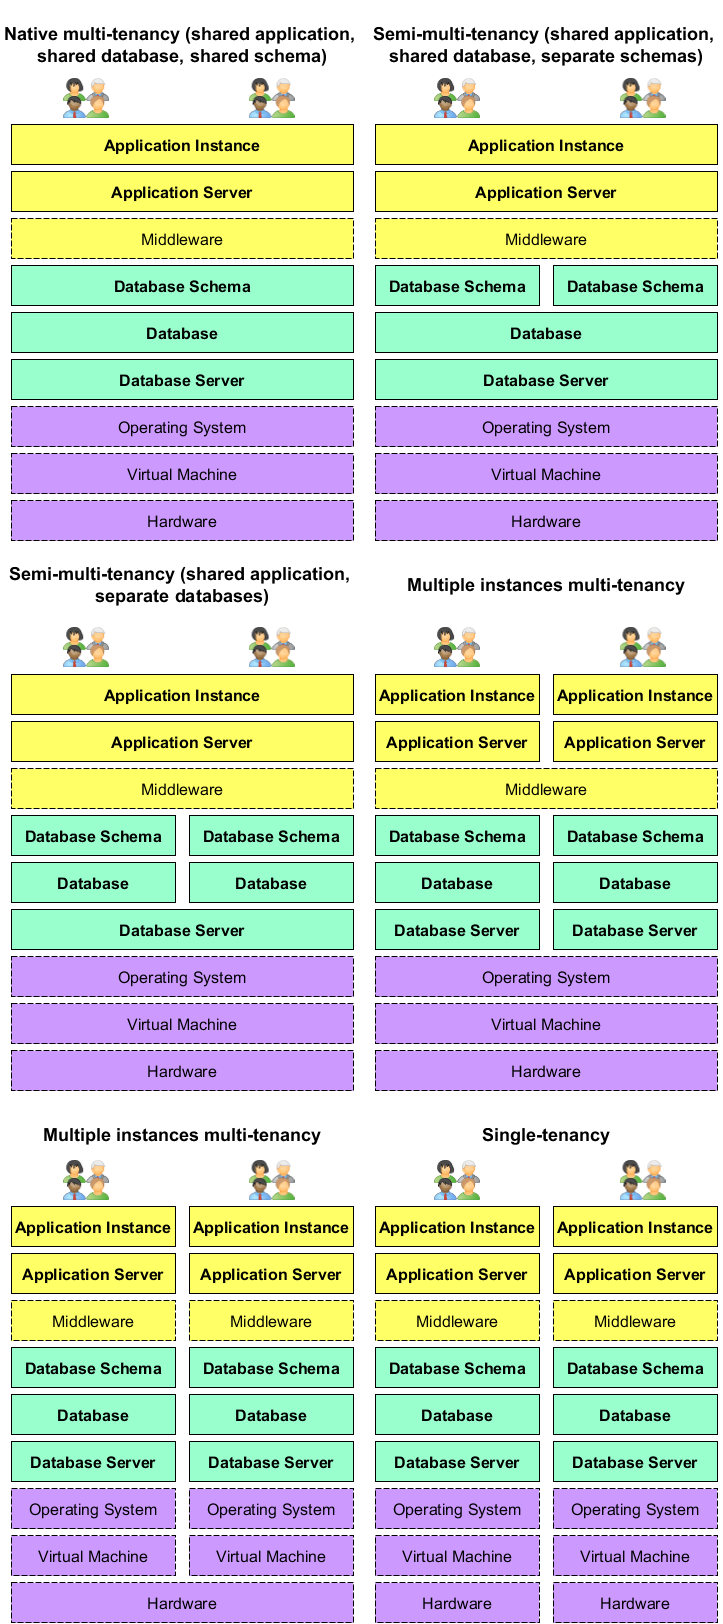
\includegraphics[max size={0.8\textwidth}{0.8\textheight}]{MTvsMILong}
	\caption{Illustration of different system levels in different variants of multi-tenancy and in single-tenancy.}
	\label{figure:MTvsMILong}
\end{figure}



\subsection{The description of the multi-tenancy variants}

In native or pure multi-tenancy \cite{Kabbedijk2015:Defining, Guo:2007:FrameworkForNative} the tenants share the same application instance and database tables which are hosted on a shared infrastructure. Native multi-tenancy variant is used to support a large number of tenants and the number is usually in the hundreds or thousands of tenants \cite{Guo:2007:FrameworkForNative}. 

In the semi-multi-tenancy variants of multi-tenancy \cite{Chong:2006:MultiTenantDataArchitecture, Bezemer:2010:MaintenanceDream} the tenants share the same application instance but the level of sharing on the database levels of the system vary. The two variants of semi-multi-tenancy are \textit{"shared application, shared database and separate schemas"}-variant and \textit{"shared application and separate databases}-variant \cite{Chong:2006:MultiTenantDataArchitecture}. 

When a high number of tenants are placed on the same server and one of the semi-multi-tenancy variants of multi-tenancy is used it can cause performance problems on the server \cite{Bezemer:2010:MaintenanceDream}. These performance problems are caused by the expensive operation of loading a database or a table in memory when a tenant accesses the application. When comparing database or table loading requirements in semi-multi-tenancy variants to native multi-tenancy native multi-tenancy enables placing more tenants on the same the server because the shared database table must be loaded only once to memory \cite{Bezemer:2010:MaintenanceDream}.

In multiple instances multi-tenancy \cite{Guo:2007:FrameworkForNative} tenants no longer share the same application instance. Instead of sharing an application instance each tenant has its own dedicated application instance over a shared middleware server, operating system or hardware \cite{Guo:2007:FrameworkForNative}. Two variants of multiple instances multi-tenancy are presented in the Figure \ref{figure:MTvsMILong}. Multiple instances multi-tenancy variants scale differently than native multi-tenancy when comparing the number of tenants which multiple instances variants or native multi-tenancy can support \cite{Guo:2007:FrameworkForNative}. Multiple instances multi-tenancy variants can support from several up to dozens of tenants on the same server while native multi-tenancy can support hundreds or thousands of tenants \cite{Guo:2007:FrameworkForNative}.

As a comparison point to different multi-tenancy variants a single-tenancy variant is also presented in the Figure \ref{figure:MTvsMILong}. In traditional single-tenant approach each tenant has its own dedicated server and own customized application instance which they use \cite{Bezemer:2010:MaintenanceDream}. This means that a single-tenant application may have many separate running instances which all can be different from each other \cite{Bezemer:2010:MaintenanceDream}. A traditional single-tenancy scenario from the early 90s was that companies moved their hardware and applications from their premises to data centers where the applications were hosted without any hardware or software sharing \cite{Guo:2007:FrameworkForNative}. 

\subsection{Multi-tenancy in Software as a Service business model}

In the academic research of multi-tenancy Software as a Service and architecture are important research topics and both of the topics are addressed a lot in multi-tenancy research \cite{Kabbedijk2015:Defining}. The frequent occurrence of those topics indicates that multi-tenancy is positioned as an architectural tactic for online software \cite{Kabbedijk2015:Defining}. 

Software as a Service is a business model where software is offered as an on-demand service for customers through Internet \cite{Bezemer:2010:MaintenanceDream}. Simplistic characterization for Software as a Service is: \textit{"Software deployed as a hosted service and accessed over the Internet"} \cite{Carraro:2006:ArchitectureLongTail}. From architectural perspective a mature and a well-designed Software as a Service application has three different attributes that separate it from a poorly designed Software as a Service application \cite{Carraro:2006:ArchitectureLongTail}. Those attributes are configurability, multi-tenant efficiency and scalability \cite{Carraro:2006:ArchitectureLongTail}.

With the help of those attributes a Software as a Service maturity model with four distinct levels can be defined \cite{Carraro:2006:ArchitectureLongTail}. Software as a Service maturity model expresses the maturity of a Software as a Service application. At each level of the maturity model one of the attributes of a mature Software as a Service application is added to the model \cite{Carraro:2006:ArchitectureLongTail}. The Figure \ref{figure:SaaSMaturity} presents the maturity model of a Software as a Service application. The attributes of a mature Software as a Service application can also be seen from the Figure \ref{figure:SaaSMaturity}. 

At the first level of the maturity model each tenant has own customized version of the application \cite{Carraro:2006:ArchitectureLongTail}. Each customized application instance is run separately on service provider's servers. At this level service providers can reduce costs by running multiple application instances on the same server hardware and by consolidating server administration \cite{Carraro:2006:ArchitectureLongTail}. Running multiple instances of the same application on the same server hardware corresponds to the multiple instances multi-tenancy variant presented in the Figure \ref{figure:MTvsMILong}. 

At the second level of the maturity model each tenant has an own separate instance of the application but all instances use the same identical code implementation \cite{Carraro:2006:ArchitectureLongTail}. At this level configurability is added to the Software as a Service application architecture so that the separate instances of the application can be configured to meet the needs of the customers \cite{Carraro:2006:ArchitectureLongTail}. Changes made to the code implementation can be delivered to all tenants. This reduces service requirements of a Software as a Service application because there is no need to upgrade individual customized instances anymore \cite{Carraro:2006:ArchitectureLongTail}. At this level the application is still served using multiple instances multi-tenancy variant.

At the third level of the maturity model multi-tenancy is added to the Software as a Service application architecture \cite{Carraro:2006:ArchitectureLongTail}. Adding multi-tenancy to the application makes it possible to run a single instance of the application on service provider's infrastructure and serve every customer using this single instance \cite{Carraro:2006:ArchitectureLongTail}. At this level the tenants are not aware of sharing the application instance with other tenants and the application instance can be customized to meet the needs of the tenants \cite{Carraro:2006:ArchitectureLongTail}. The resources needed to host a single instance of an application on the level three are lower than the resources needed for multiple instances on levels one and two which lowers the costs of hosting the application \cite{Carraro:2006:ArchitectureLongTail}. The disadvantage of the single instance multi-tenant approach at this level is that when the amount of tenants increases the only way to scale the application up is to host it on a more powerful server \cite{Carraro:2006:ArchitectureLongTail}. 

At the fourth level of the maturity model scalability is added to the Software as a Service application architecture \cite{Carraro:2006:ArchitectureLongTail}. At this level the use of a tenant load balancer enables adding and removing application servers and instances according to the current demand \cite{Carraro:2006:ArchitectureLongTail}.

\begin{figure}
	\centering
		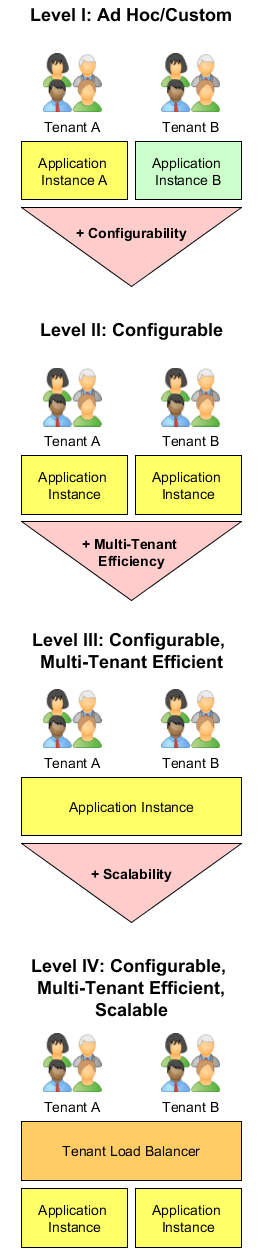
\includegraphics[max size={0.9\textwidth}{0.9\textheight}]{SaaSMaturity}
	\caption{The levels of the Software as a Service maturity model.}
	\label{figure:SaaSMaturity}
\end{figure}



\section{Characteristics of multi-tenancy}

There are three different characteristics of multi-tenancy that are often mentioned when describing multi-tenancy in scientific literature. Those characteristics that are used to describe multi-tenancy are sharing of hardware resources, possibility to configure the shared application instance in runtime and shared application and database instances \cite{Bezemer:2010:MaintenanceDream}. The definition of multi-tenancy proposed by Kabbedijk et al. \cite{Kabbedijk2015:Defining} also mentions all of these characteristics of multi-tenancy. 

When applications are served to customers as single-tenant applications server utilization can be low especially when applications are used by customers in the small and medium enterprise (SME) segment of the market \cite{Bezemer:2010:MaintenanceDream}. In that situation server utilization can be improved by placing several tenants on the same server \cite{Bezemer:2010:MaintenanceDream}. Different multi-tenancy variants from multiple instances multi-tenancy to native multi-tenancy can be used to place several tenants on the same server. Placing several tenants on the same server improves the utilization of the servers \cite{Bezemer:2010:MaintenanceDream}. 

Through higher utilization of the servers the total amount of hardware required to serve the tenants is lower than when using single-tenancy where each tenant has its own dedicated server. The result of requiring lower amount of hardware because of higher server utilization in multi-tenancy is that the overall delivery costs of the application will be lower \cite{Bezemer:2010:MaintenanceDream}. The reduced delivery costs make it possible for the service provider to improve the profit margin and to offer the service to the customers at lower service subscription costs \cite{Guo:2007:FrameworkForNative}.

Sharing the same hardware resources can also cause problems in addition to the benefits of sharing the same resources. In a situation where the hardware resources are shared a problem caused by one tenant can affect all the other tenants that use the same shared resources \cite{Bezemer:2010:EnablingMultiTenancy}. In such a situation when one tenant blocks the resources the performance of all other tenants can be compromised \cite{Bezemer:2010:MaintenanceDream}. 

In multi-tenancy tenants should be able to make customizations to their own application in runtime without impacting other tenants \cite{Guo:2007:FrameworkForNative}. In addition to multi-tenant and multiple instances multi-tenancy concepts there is also a third software system concept namely multi-user concept \cite{Bezemer:2010:MaintenanceDream}. One difference between multi-tenant and multi-user concepts is that in multi-tenancy each tenant can configure for example the appearance or the workflow of the application heavily \cite{Bezemer:2010:MaintenanceDream}. In multi-user applications all customers use the same application and have only limited configuration options \cite{Bezemer:2010:MaintenanceDream}. This means that in multi-user concept the application functionality is the same for all customers but the application can be still partly configurable \cite{Kabbedijk2015:Defining}. 

Introducing configurability in a multi-tenant application can result in more complex application code \cite{Bezemer:2010:EnablingMultiTenancy}. In single-tenancy application configuration can be done by creating a branch in the development tree and deploying a separate instance of the application \cite{Bezemer:2010:MaintenanceDream}. In multi-tenancy the possibility to configure the application is integrated in the application architecture which increases the code complexity \cite{Bezemer:2010:MaintenanceDream}. Increased code complexity can cause problems in the maintenance phase of the application \cite{Bezemer:2010:MaintenanceDream}. 

The third characteristic of multi-tenancy is the ability to share one application and database instance. In native and semi-multi-tenancy variants of multi-tenancy the application instance is shared among different tenants which can be seen from the Figure \ref{figure:MTvsMILong}. In native multi-tenancy also the database and schema are shared among tenants. When the data of all of the tenants is on the same server it can cause risks in terms of security \cite{Bezemer:2010:EnablingMultiTenancy}. A security breach can cause the exposure of one tenant's data to other tenants \cite{Bezemer:2010:MaintenanceDream}. Therefore the protection of each tenant's critical information is an important topic in multi-tenancy \cite{Guo:2007:FrameworkForNative}.



\section{Discussion}

The definition of multi-tenancy used in this seminar paper is the definition which Kabbedijk et al. present in their paper \textit{"Defining multi-tenancy: A systematic mapping study on the academic and the industrial perspective"} \cite{Kabbedijk2015:Defining}. This definition was chosen for this seminar paper because it is clear and comprehensive and is based on scientific research of several different multi-tenancy definitions. Answers to the research questions one and two can be found in the Section 3 where the definition of multi-tenancy and the connection between multi-tenancy and Software as a Service business model are presented. 

In the different variants of multi-tenancy presented in the Section 3 multi-tenancy is applied to different levels of the system. In the multiple instances multi-tenancy variant only the hardware or the operating system levels are shared among different tenants while each tenant has its own dedicated application instance. When using semi-multi-tenancy the amount of sharing on the database level of the system vary from shared database and separate schemas to separate databases. The highest level of sharing is achieved in native multi-tenancy where all system levels are shared among all tenants. 

This seminar paper does not provide a concrete example of a multi-tenant Software as a Service application. In order to provide a deeper description of the different variants of multi-tenancy some concrete examples of multi-tenant applications and their differences could have been useful. 

Since Software as a Service is a frequent topic in the academic research of multi-tenancy and multi-tenancy is part of the Software as a Service maturity model the connection between multi-tenancy and Software as a Service business model is strong. With the help of multi-tenancy service provider can achieve savings in application maintenance and server infrastructure costs by maintaining only a single code base for the application and hosting only a single instance of an application on his or her server infrastructure. 

Some of the challenges caused by the characteristics of multi-tenancy are presented in the Section 4. The characteristics of multi-tenancy can cause challenges in the performance, maintenance and security areas of the application. When developing multi-tenant applications it would be good to take those challenges into consideration in order to mitigate the problems that the challenges can cause. This seminar paper discusses only some of the challenges of multi-tenancy and there can be other challenges which are not mentioned in this seminar paper.

One limitation that affects the validity of this seminar paper is that the author has never, at least not knowingly, used a real multi-tenant application or researched the architecture of a real multi-tenant application. The consequence of this limitation is that the author's interpretations of multi-tenancy and the variants of multi-tenancy are only based on scientific literature without real industrial experience of multi-tenancy. 

\section{Conclusion}

In this paper the different variants of multi-tenancy in scientific literature were illustrated from the perspective of Software as a Service business model. Multi-tenancy is a high level architectural pattern which can be used to reduce service provider's overall delivery costs of the application in order to improve the profit margin. The reduced delivery costs make it also possible for the service provider to offer the service to the customers at lower service subscription costs. Multi-tenancy is one of the attributes of a mature well-defined Software as a Service application. The topic of Software as a Service is also addressed a lot in the academic research of multi-tenancy. In addition to the benefits of multi-tenancy the characteristics of multi-tenancy can cause challenges in the performance, maintenance and security areas of the application. Those challenges need to be taken into consideration when developing multi-tenant applications in order to mitigate the problems caused by those challenges. 





% trigger a \newpage just before the given reference
% number - used to balance the columns on the last page
% adjust value as needed - may need to be readjusted if
% the document is modified later
%\IEEEtriggeratref{8}
% The "triggered" command can be changed if desired:
%\IEEEtriggercmd{\enlargethispage{-5in}}

% references section

% can use a bibliography generated by BibTeX as a .bbl file
% BibTeX documentation can be easily obtained at:
% http://mirror.ctan.org/biblio/bibtex/contrib/doc/
% The IEEEtran BibTeX style support page is at:
% http://www.michaelshell.org/tex/ieeetran/bibtex/
%\bibliographystyle{IEEEtran}
% argument is your BibTeX string definitions and bibliography database(s)
%\bibliography{IEEEabrv,../bib/paper}
%
% <OR> manually copy in the resultant .bbl file
% set second argument of \begin to the number of references
% (used to reserve space for the reference number labels box)



%\begin{thebibliography}{1}
%
%\bibitem{IEEEhowto:kopka}
%H.~Kopka and P.~W. Daly, \emph{A Guide to \LaTeX}, 3rd~ed.\hskip 1em plus
%  0.5em minus 0.4em\relax Harlow, England: Addison-Wesley, 1999.
%

\bibliographystyle{IEEEtran}
\bibliography{IEEEabrv,sasmoota2017}
%\end{thebibliography}




\end{document}


